\documentclass{article}%
\usepackage[T2A,T1]{fontenc}%
\usepackage[utf8]{inputenc}%
\usepackage{geometry}%
\geometry{tmargin=20mm,bmargin=20mm,lmargin=20mm,rmargin=20mm}%
\usepackage{newtxtext, newtxmath}%
\usepackage{substitutefont}%
\usepackage{lastpage}%
\usepackage{ragged2e}%
\usepackage{graphicx}%
\usepackage{amsmath}%
\usepackage{subcaption}%
\usepackage{fancyhdr}%
%
\linespread{1.5}%
\usepackage{newunicodechar}%
\fancypagestyle{header}{%
\renewcommand{\headrulewidth}{0.5pt}%
\renewcommand{\footrulewidth}{1.0pt}%
\fancyhead{%
}%
\fancyfoot{%
}%
\fancyhead[C]{%
CALCULATION SHEET%
}%
\fancyfoot[L]{%
H{-}MAX603{-}CAL{-}MM{-}18SKIP{-}001{-}SHT{-}001%
}%
\fancyfoot[R]{%
Page \thepage\ of \pageref{LastPage}%
}%
}%
%
\begin{document}%
\pagestyle{empty}%
\normalsize%
\pagestyle{header}%
\begin{center}%
\section*{}%
\label{sec:}%
\begin{minipage}{\textwidth}%
\centering%
\begin{Large}%
\textbf{HOLT CONSULTING ENGINEERS (PTY) LTD}%
\end{Large}%
\vspace*{20pt}%
\linebreak%
\begin{large}%
\textbf{TUMELA 18 TON SKIP DESIGN}%
\end{large}%
\vspace*{20pt}%
\linebreak%
\begin{large}%
\textbf{H{-}MAX603}%
\end{large}%
\vspace*{20pt}%
\linebreak%
\begin{large}%
\textbf{H{-}MAX603{-}CAL{-}MM{-}18SKIP{-}001{-}SHT{-}001}%
\end{large}%
\vspace*{80pt}%
\end{minipage}

%
\end{center}%
\begin{center}%
\begin{minipage}{\textwidth}%
\flushleft%
\begin{tabular}{|l |l |}%
\hline%
\textbf{Engineer:}&Gerald Holt (Pr.Eng)\\%
\cline{1%
-%
2}%
\textbf{Registration:}&20020259\\%
\cline{1%
-%
2}%
\textbf{Email:}&gerald@holtconsulting.co.za\\%
\cline{1%
-%
2}%
\textbf{Phone:}&+27{-}791{-}2549\\%
\cline{1%
-%
2}%
\textbf{Adress:}&Unit G, Mini Park\\%
\cline{1%
-%
2}%
\textbf{}&16 Gerhardus Street, Strijdom Park\\%
\cline{1%
-%
2}%
\textbf{}&Randburg, South Africa\\%
\cline{1%
-%
2}%
\textbf{Website:}&www.holtconsulting.co.za\\%
\cline{1%
-%
2}%
\end{tabular}%
\vspace*{150pt}%
\centering%
\end{minipage}%
\end{center}%


\begin{figure}[h!]%

\includegraphics[width=240px]{HCE.jpg}%
\centering%
\end{figure}

%
\newpage%
\begin{center}%
\section*{REVISION HISTORY}%
\label{sec:REVISIONHISTORY}%

%
\begin{minipage}{\textwidth}%
\centering%
\begin{tabular}{|c |c |c |c |c |c |}%
\hline%
\textbf{REV}&\textbf{DESCRIPTION}&\textbf{DATE}&\textbf{ISSUED BY}&\textbf{REVIEWED BY}&\textbf{APPROVED}\\%
\hline%
A&ISSUED FOR REVIEW&2022{-}10{-}15&G.G. HOLT&H.F. HOLT&\\%
\hline%
\end{tabular}%
\end{minipage}%
\end{center}%
\newpage%
\section{CUSTOMER DETAILS}%
\label{sec:CUSTOMERDETAILS}%
\begin{flushleft}%
\begin{minipage}{\textwidth}%
\centering%
\begin{tabular}{|l |l |}%
\hline%
\textbf{Customer:}&Max Power Services (Pty) Ltd\\%
\cline{1%
-%
2}%
\textbf{Customer Name:}&Herman de Koker\\%
\cline{1%
-%
2}%
\textbf{Customer Email:}&harry@maxpower.co.za\\%
\cline{1%
-%
2}%
\end{tabular}%
\end{minipage}%
\end{flushleft}

%
\newpage%
\section{CALCULATION INPUT DATA}%
\label{sec:CALCULATIONINPUTDATA}%
\subsection{Applicable Design Codes}%
\label{subsec:ApplicableDesignCodes}%
\begin{flushleft}%
SANS 10208: 3 {-} 2017: Design of structures for the mining industry Part 3: Conveyances%
\linebreak%
SANS 10610: Buildling loading code%
\linebreak%
SANS 10162: Steel design%
\linebreak%
\end{flushleft}

%
\subsection{General Data}%
\label{subsec:GeneralData}%
\begin{flushleft}%
\begin{minipage}{\textwidth}%
\flushleft%
\begin{tabular}{|l |l |c|}%
\hline%
\textbf{Design Method}&Limit States (Rope Break Conditions)&\\%
\hline%
\textbf{Material of Construction}&Main Body: EN10025 S355JR&\\%
\hline%
\textbf{Material of Construction}&Liners: VRN 500&\\%
\hline%
\textbf{Yield Stress}&355&$MPa$\\%
\hline%
\textbf{Skip Weight}&9878&$kg$\\%
\hline%
\textbf{Payload}&18000&$kg$\\%
\hline%
\textbf{Winding Speed}&15&$m/s$\\%
\hline%
\textbf{Winding Rope Diameter}&54&$mm$\\%
\hline%
\textbf{Winding Rope Unit Mass}&12.45&$kg/m$\\%
\hline%
\textbf{Rope Break Force}&2319&$kN$\\%
\hline%
\textbf{Ultimate Tensile Strength}&1900&$MPa$\\%
\hline%
\textbf{Winder Acceleration}&0.8&$m/s^2$\\%
\hline%
\textbf{Winder Trip Acceleration}&5&$m/s^2$\\%
\hline%
\textbf{Winder Travel Distance}&1023&$m$\\%
\hline%
\textbf{Number of Cycles per Month}&3000&\\%
\hline%
\textbf{Skip Internal Height}&5600&$mm$\\%
\hline%
\textbf{Skip Internal Width}&1557&$mm$\\%
\hline%
\textbf{Skip Internal Depth}&1400&$mm$\\%
\hline%
\textbf{Skip Overall Height}&10713&$mm$\\%
\hline%
\textbf{Skip Overall Width}&1856&$mm$\\%
\hline%
\textbf{Skip Overall Depth}&1743&$mm$\\%
\hline%
\textbf{Ore Bulk Density}&1950&$kg/m^3$\\%
\hline%
\end{tabular}%
\end{minipage}%
\end{flushleft}

%
\newpage%
\subsection{Assumption Data}%
\label{subsec:AssumptionData}%
\begin{flushleft}%
\begin{minipage}{\textwidth}%
\flushleft%
\begin{tabular}{|l |l |l|}%
\hline%
\textbf{Spacing between rails}&1800&$mm$\\%
\hline%
\textbf{Top Hat Guide Specification}&340 x 175mm&\\%
\hline%
\textbf{Top Hat Guide Material Specification}&EN10025 S355JR&\\%
\hline%
\textbf{Top Hat Guide Unit Mass}&85.95&$kg/m$\\%
\hline%
\textbf{Top Hat Guide Width}&175&$mm$\\%
\hline%
\textbf{Bunton Stiffness}&1608000&$N/m$\\%
\hline%
\textbf{Guide Stiffnes}&1600000&$N/m$\\%
\hline%
\end{tabular}%
\end{minipage}%
\end{flushleft}

%
\newpage%
\subsection{Sketches and Drawings}%
\label{subsec:SketchesandDrawings}%
\subsubsection{General Arrangement}%
\label{ssubsec:GeneralArrangement}%


\begin{figure}[h!]%
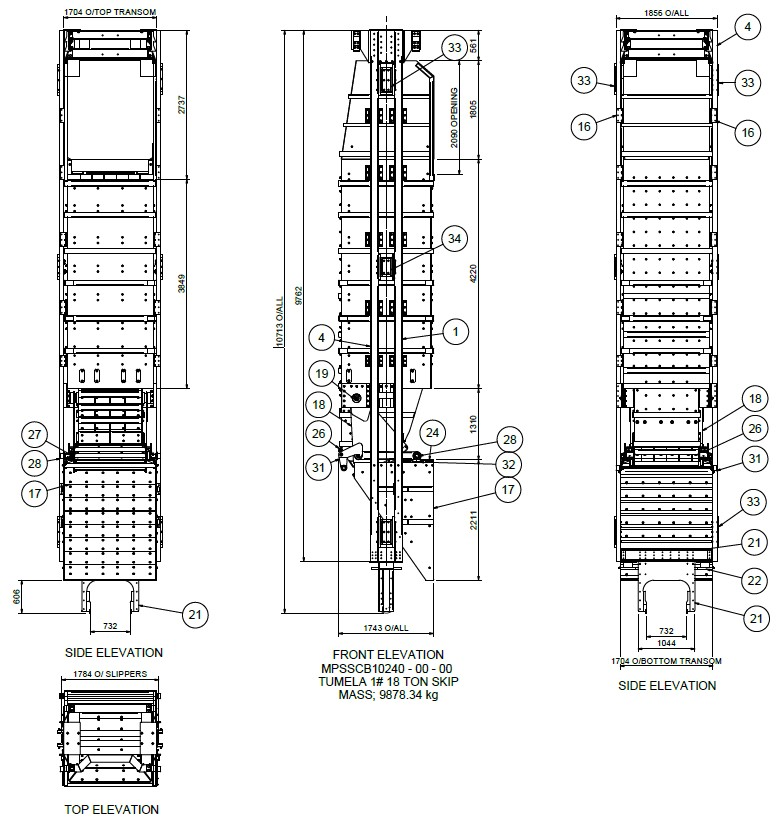
\includegraphics[width=380px]{Tumela 18 ton Skip.jpg}%
\centering%
\caption{18 ton Skip Drawing}%
\centering%
\end{figure}

%
\newpage%
\subsubsection{Isometric Views}%
\label{ssubsec:IsometricViews}%


\begin{figure}[h!]%
\begin{subfigure}[b]{0.45\linewidth}%
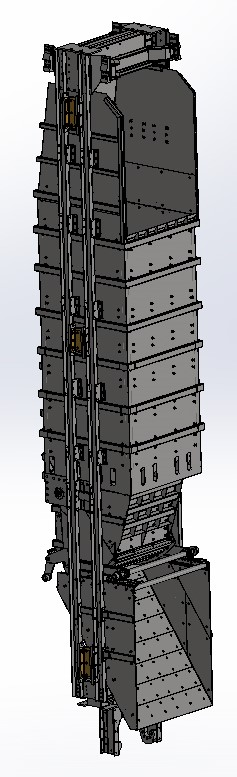
\includegraphics[width=130px]{Tumela 18 ton Skip_iso_1.jpg}%
\centering%
\caption{18 ton Skip Isometric View 1}%
\end{subfigure}%
\begin{subfigure}[b]{0.45\linewidth}%
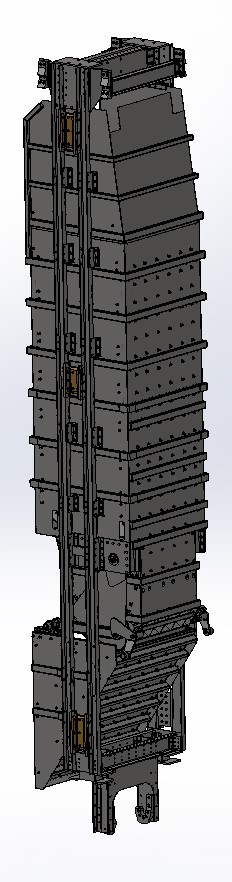
\includegraphics[width=120px]{Tumela 18 ton Skip_iso_3.jpg}%
\centering%
\caption{18 ton Skip Isometric View 3}%
\end{subfigure}%
\end{figure}

%
\newpage

%
\section{CALCULATIONS}%
\label{sec:CALCULATIONS}%
\subsection{Skip Loads}%
\label{subsec:SkipLoads}%
\subsubsection{Basic Skip Parameters}%
\label{ssubsec:BasicSkipParameters}%
\begin{flushleft}%
\begin{minipage}{\textwidth}%
\flushleft%
\begin{tabular}{l l l l}%
Payload&$R$&18000&$kg$\\%
Payload&$R_l$&176580.0&$N$\\%
Winding Speed&$V_w$&15&$m/s$\\%
Winder Acceleration&$a_w$&0.8&$m/s^2$\\%
Winder Trip Acceleration&$a_t$&5&$m/s^2$\\%
Winding Rope Diameter&$Rope_d$&54&$m/s^2$\\%
Rope Break Force&$RBF$&2319&$kN$\\%
Ultimate Tensile Strength&$UTS$&1900&$MPa$\\%
Ore Bulk Density&$\rho_b$&1950&$kg/m^3$\\%
Skip Internal Width&$b$&1557&$mm$\\%
Skip Internal Depth&$w$&1557&$mm$\\%
Skip Volume Required&$Vol = R / \rho_b$&9.2&$m^3$\\%
Ore Height in Skip&$h = Vol/(b w)$&4.2&$m$\\%
Rope Strentch Under Payload&$\Delta L$&765.8&$mm$\\%
\end{tabular}%
\end{minipage}%
\end{flushleft}

%
\subsubsection{Permanent Loads}%
\label{ssubsec:PermanentLoads}%
\begin{flushleft}%
\begin{minipage}{\textwidth}%
\flushleft%
\begin{tabular}{l l l l}%
Skip Bridle Sides&$m_1$&1167&$kg$\\%
Skip Bridle Top Transom&$m_2$&1522&$kg$\\%
Skip Bridle Bottom Transom&$m_3$&850&$kg$\\%
Skip Unit&$m_4$&6336&$kg$\\%
Permanent Load&$G_c = (m_1 + m_3 + m_4)g$&81943&$N$\\%
\end{tabular}%
\end{minipage}%
\end{flushleft}%


\begin{figure}[h!]%
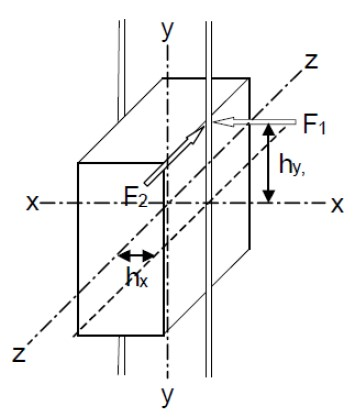
\includegraphics[width=180px]{Force_diagram.jpg}%
\centering%
\caption{Properties Diagram}%
\centering%
\end{figure}

%
\subsubsection{Laterial Imposed Loads (H) {-} Fixed Guide Systems in Vertical Shafts}%
\label{ssubsec:LaterialImposedLoads(H){-}FixedGuideSystemsinVerticalShafts}%
\begin{flushleft}%
\begin{minipage}{\textwidth}%
\flushleft%
\begin{tabular}{l l l l}%
Clearance between Roller and Slipper&$\Delta_c$&10&$mm$\\%
Slipper Plate Impact Factor&$\alpha_n$&2&\\%
Guide Roller Assembly Stiffness&$k_r$&500000&$N/m$\\%
Bunton Stiffness&$k_b$&1608000&$N/m$\\%
Guide Stiffnes&$k_g$&1600000&$N/m$\\%
Moment of Inertia about X{-}axis&$I_x$&80510&$kg.m^2$\\%
Moment of Inertia about Y{-}axis&$I_y$&6838&$kg.m^2$\\%
Moment of Inertia about Z{-}axis&$I_z$&82050&$kg.m^2$\\%
Distance from slipper to center of gravity&$h_x$&892&$mm$\\%
Distance from slipper to center of gravity&$h_y$&4847&$mm$\\%
Distance from slipper to center of gravity&$h_z$&28&$mm$\\%
Guide Roller Lateral Load&$H_f$&5000000&$N$\\%
Steelwork Stiffness Ratio&$r_k$&1.005&$ $\\%
Weight of Skip System&$m_c$&8353&$kg$\\%
Effective Mass About y {-} x Plane&$m_x = (m_c I_z) / (I_z + m_c (h_y)^2)$&2463.0&$kg$\\%
Effective Mass About y {-} z Plane&$m_z = (m_c I_x I_y)/(I_x I_y +(m_c I_x (h_y)^2) + (m_c I_y (h_x)^2)$&280.0&$kg$\\%
Non{-}Dimensional Laterial Stiffness&$K_x = (k_b L_b^2)/m_x V^2$&9&\\%
Non{-}Dimensional Laterial Stiffness&$K_z = (k_b L_b^2)/m_z V^2$&83&\\%
Plate Coefficient from graph&$P_b$&0.05&\\%
Maximum Moving Misalighnment&$e$&0.01&$m$\\%
Lateral Slipper Pad Load&$H_s$&7791&$N$\\%
\end{tabular}%
\end{minipage}%
\end{flushleft}%


\begin{figure}[h!]%
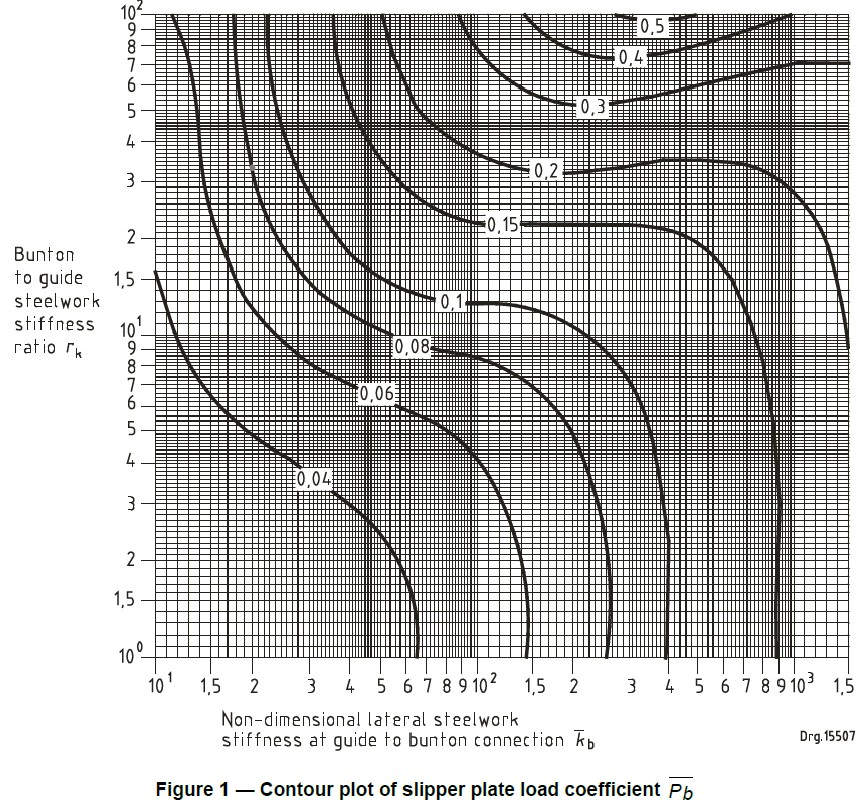
\includegraphics[width=360px]{plate_load_coef.jpg}%
\centering%
\caption{Slipper Plate Load Coefficient Pb}%
\centering%
\end{figure}

%
\subsubsection{Winder System Loads}%
\label{ssubsec:WinderSystemLoads}%
\begin{flushleft}%
\begin{minipage}{\textwidth}%
\flushleft%
\begin{tabular}{l l l l}%
Dynamic Impact Factor&$\alpha_d$&2&\\%
Winder Acceleration and Deceleration&$a_o$&0.8&$m/s^2$\\%
Winder Trip Acceleration&$a_t$&0.8&$m/s^2$\\%
Skip Self Weight&$G_c$&81943&$N$\\%
Content Load&$C_y$&176580.0&$N$\\%
Tail Rope Load&$T$&0&$N$\\%
Acceleration Load&$A_o = (\alpha_d) a_o (G_c + C_y + T)/g$&42165&$N$\\%
Acceleration Trip Out Load&$A_t = (\alpha_d) a_t (G_c + C_y + T)/g$&263530&$N$\\%
\end{tabular}%
\end{minipage}%
\end{flushleft}

%
\subsubsection{Emergency Loads}%
\label{ssubsec:EmergencyLoads}%
\begin{flushleft}%
\begin{minipage}{\textwidth}%
\flushleft%
\begin{tabular}{l l l l}%
Emergency Load&$E_r$&2319000&$N$\\%
\end{tabular}%
\end{minipage}%
\end{flushleft}

%
\subsubsection{Vertical Friction Loads}%
\label{ssubsec:VerticalFrictionLoads}%
\begin{flushleft}%
\begin{minipage}{\textwidth}%
\flushleft%
\begin{tabular}{l l l l}%
Lateral Slipper Pad Load&$H_s$&7791&$N$\\%
Vertical Friction Load&$F_v = 0.5 H_s$&3895.5&$N$\\%
\end{tabular}%
\end{minipage}%
\end{flushleft}

%
\subsubsection{Rock Loads}%
\label{ssubsec:RockLoads}%
\begin{flushleft}%
\begin{minipage}{\textwidth}%
\flushleft%
\begin{tabular}{l l l l}%
Filling Impact Factor in Stationary Position&$\alpha_v$&1.5&\\%
Load on Tipping Rollers Impact Factor&$\alpha_t$&2&\\%
Static Load&$R$&176580.0&$N$\\%
Bridle Transom Load While Filling&$R_d = (\alpha_v)(R)$&27000.0&$N$\\%
Rock Pressure&$p_o = \rho_b g h$&80.3439&$N/m^2$\\%
Pressure on the Door&$p_1 = 1 p_o$&80.3&$N/m^2$\\%
Pressure on the Back of Skip&$p_2 = 0.5 p_o$&40.2&$N/m^2$\\%
Pressure on the Lower Portion Skip Back&$p_3 = 0.5 p_o$&120.5&$N/m^2$\\%
Pressure on the Front and Sides of Skip&$p_4 = 0.2 p_o$&16.1&$N/m^2$\\%
\end{tabular}%
\end{minipage}%
\end{flushleft}

%
\subsection{Skip Element Design}%
\label{subsec:SkipElementDesign}%
\subsubsection{Top Transom}%
\label{ssubsec:TopTransom}%


\begin{figure}[h!]%
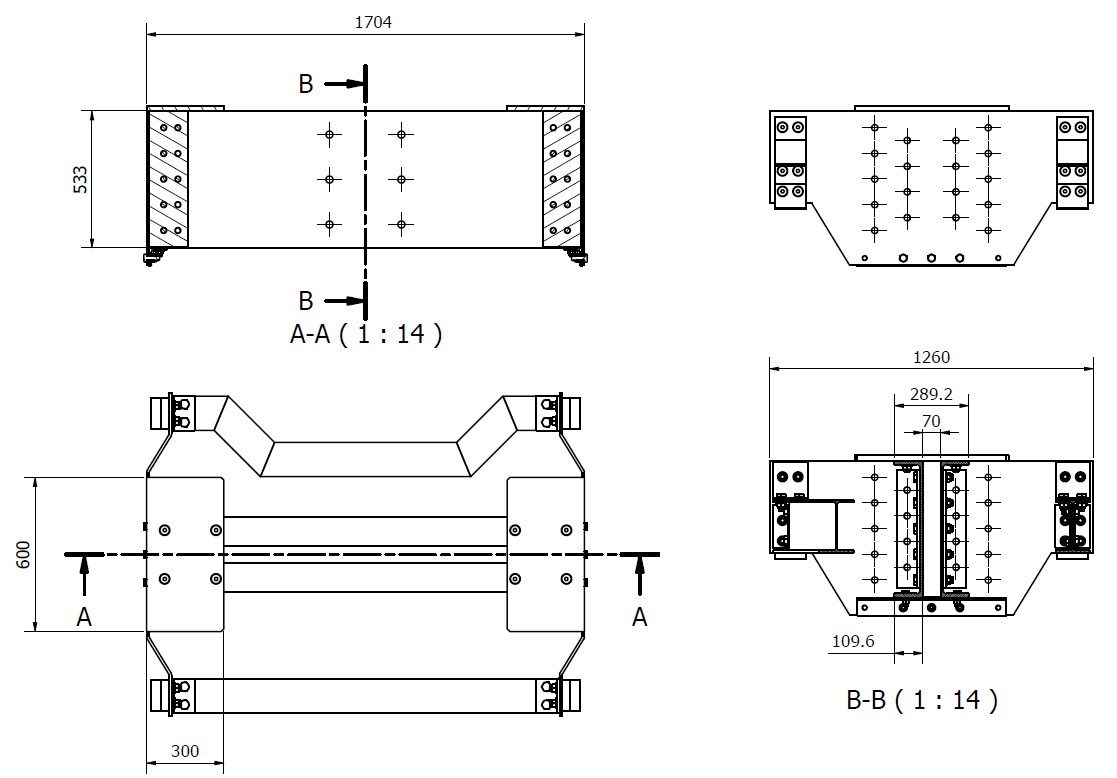
\includegraphics[width=360px]{Top_Transom.jpg}%
\centering%
\caption{Top Transom Configuration}%
\centering%
\end{figure}

%
\newpage%
\textbf{Material Data}%
\newline%
%
2 / 533 x 110 CHANNEL (MODIFIED 533 X 210 X 93 UB) WITH TOP AND BOTTOM 20 X 100 PLATE%
\newline%
%
4 / 20 X 100 PLATES (TOP AND BOTTOM)%
\newline%
%
2 / 150 x 150 ANGLE END CONNECTIONS%
\begin{flushleft}%
\begin{minipage}{\textwidth}%
\flushleft%
\begin{tabular}{l l l l}%
Length of Transom&$L$&1700&$mm$\\%
Channel Width&$b$&109&$mm$\\%
Channel Height&$h$&533&$mm$\\%
Channel Web Thickness&$t_w$&10.2&$mm$\\%
Channel Flange Thickness&$t_f$&15.6&$mm$\\%
Top and Bottom Plate Width&$w$&110&$mm$\\%
Top and Bottom Plate Thickness&$t_p$&20&$mm$\\%
Yield Stress&$f_y$&355&$MPa$\\%
Channel Cross Sectional Area&$A=2bt_f + h_w*t_w$&8519.0&$mm^2$\\%
Channel Centroid Distance&$x_c=(0.5h_wt_w^2 + t_fb^2)/A$&25.0&$mm$\\%
Channel Second Moment of Area about x{-}x&$I_x=bh^3/12 - b_fh_w^3/12$&335071491.0&$mm^4$\\%
Channel Second Moment of Area about y{-}y&$I_y=h_wt_w^3/3+2t_fb^3/3 - Ax_c^2)$&8397644.0&$mm^4$\\%
Double Plate Polar Moment&$J = I_x + I_y$&340973234.0&$mm^4$\\%
Channel Warping Constant&$C_w = (1/144)(t_f^3b^3)+(1/36)(h - t_f/2)^3)t_w^3$&4304577645.0&$mm^6$\\%
Channel Plastic Section Modulus&$Z_p=bh^2/4 - b_fh_w^2/4$&1521885.0&$mm^3$\\%
Double Plate Cross Sectional Area&$A = 2(wt_p)$&4400&$mm^2$\\%
Double Plate Second Moment of Area about x{-}x&$I_x = w/12(H^3-h^3)$&336536567.0&$mm^4$\\%
Double Plate Second Moment of Area about y{-}y&$I_y = t_pw^3/6$&4436667.0&$mm^4$\\%
Double Plate Plastic Section Modulus&$Z_p = 2(wt_p(h-t_p/2)$&2301200.0&$mm^3$\\%
Combined Second Moment of Area about x{-}x&$I_x$&671608058.0&$mm^3$\\%
Combined Second Moment of Area about y{-}y&$I_y$&12834311.0&$mm^3$\\%
Combined Plastic Section Modulus&$Z_p$&3823085.0&$mm^3$\\%
Plastic Moment&$M_p = Z_pf_y$&1357.2&$kNm$\\%
Adjusted Plastic Moment&$0.67M_p$&909.3&$kNm$\\%
Critical Elastic Moment&$M_c = ((\pi^4E^2C_wI_y)/L^4 + (\pi^2EI_yGJ)/L^2)^0.5$&20494.3&$kNm$\\%
Factored Moment Resistance&$M_r = 1.15 \phi M_p(1-(0.28M_p/M_c))$&1378.7&$kNm$\\%
Factored Shear Resistance&$Vr = 0.55 \phi A f_y$&2270.0&$kNm$\\%
\end{tabular}%
\end{minipage}%
\end{flushleft}%
\textbf{Design for Emergency Loads}%
\begin{flushleft}%
\begin{minipage}{\textwidth}%
\flushleft%
\begin{tabular}{l l l l}%
Rope Break Force&$RBF$&2319&$kN$\\%
Number of Beams&$No.$&2&\\%
Combined Shear Resistance&$M_r$&4540.0&$kN$\\%
Ultimate Bending Moment&$M_u = RBF L/4$&986.0&$kN$\\%
Ultimate Shear Force&$M_u = RBF/2$&1160.0&$kN$\\%
Interaction Check&$M_u/M_r + V_u/V_r < 1$&0.61&$Pass$\\%
\end{tabular}%
\end{minipage}%
\end{flushleft}%
\textbf{Design for Operation Loads}%
\begin{flushleft}%
\begin{minipage}{\textwidth}%
\flushleft%
\begin{tabular}{l l l l}%
Operation Force&$LC = 1.2G_c + 1.6R$&127.0&$kN$\\%
Number of Beams&$No.$&2&\\%
Combined Shear Resistance&$M_r$&4540.0&$kN$\\%
Ultimate Bending Moment&$M_u = (RBF) L/4$&54.0&$kN$\\%
Ultimate Shear Force&$M_u = (RBF)/2$&64.0&$kN$\\%
Interaction Check&$M_u/M_r + V_u/V_r < 1$&0.03&$Pass$\\%
\end{tabular}%
\end{minipage}%
\end{flushleft}%
\textbf{Design for Fatigue Loads}%
\begin{flushleft}%
\begin{minipage}{\textwidth}%
\flushleft%
\begin{tabular}{l l l l}%
Cycles per Month&$Cycles$&3000&\\%
Design Life&$Design$&24&$months$\\%
Total Number of Trips&$Trips$&72000&\\%
Rock during Filling&$R_d = (\alpha_v)(R)$&27000.0&$N$\\%
Permanent Load&$G_c = (m_1 + m_3 + m_4)g$&81943&$N$\\%
Major Cycle Load&$MCL = R_d + 0.25G_c$&47485.75&$N$\\%
Stress Amplitude&$\sigma_a = 0.5 (MCL) L/(4 Z_p))$&2.65&$MPa$\\%
Acceleration Cycles Load&$2A_o$&84330&$N$\\%
Stress Acceleration Increase&$\sigma_b = 0.5 (2 A_o L/(4 Z_p))$&9.4&$MPa$\\%
Bounding Load&$0.2R$&3600.0&$N$\\%
Stress Acceleration Increase&$\sigma_c = 0.5 (0.2 R L/(4 Z_p))$&0.4&$MPa$\\%
Steel Endurance Limit&$S_e$&70&$MPa$\\%
Interaction Check&$\sigma_a/S_e + \sigma_b/S_e + \sigma_c/S_e < 1$&0.11&$Pass$\\%
\end{tabular}%
\end{minipage}%
\end{flushleft}

%
\newpage%
\subsubsection{Bottom Transom}%
\label{ssubsec:BottomTransom}%


\begin{figure}[h!]%
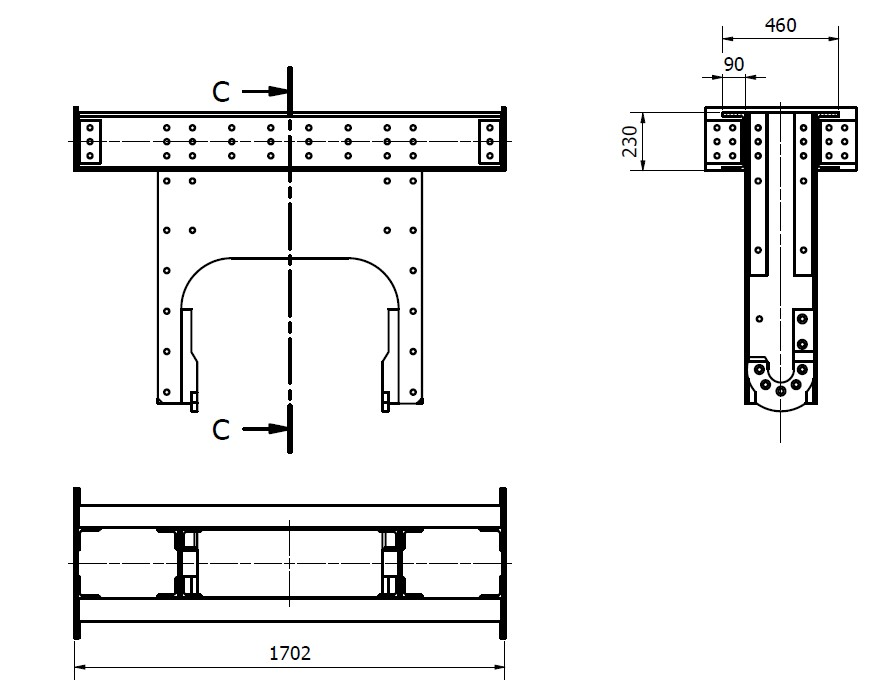
\includegraphics[width=360px]{Bottom_Transom.jpg}%
\centering%
\caption{Bottom Transom Configuration}%
\centering%
\end{figure}

%
\textbf{Material Data}%
\newline%
%
2 / 230 x 90 CHANNEL%
\newline%
%
4 / 20 X 230 PLATES (TOP AND BOTTOM)%
\newline%
%
2 / 100 x 100 ANGLE END CONNECTIONS%
\begin{flushleft}%
\begin{minipage}{\textwidth}%
\flushleft%
\begin{tabular}{l l l l}%
Length of Transom&$L$&1700&$mm$\\%
Channel Width&$b$&90&$mm$\\%
Channel Height&$h$&230&$mm$\\%
Channel Web Thickness&$t_w$&7.5&$mm$\\%
Channel Flange Thickness&$t_f$&14&$mm$\\%
Top and Bottom Plate Width&$w$&230&$mm$\\%
Top and Bottom Plate Thickness&$t_p$&20&$mm$\\%
Yield Stress&$f_y$&355&$MPa$\\%
Channel Cross Sectional Area&$A=2bt_f + h_w*t_w$&4035.0&$mm^2$\\%
Channel Centroid Distance&$x_c=(0.5h_wt_w^2 + t_fb^2)/A$&30.0&$mm$\\%
Channel Second Moment of Area about x{-}x&$I_x=bh^3/12 - b_fh_w^3/12$&34585945.0&$mm^4$\\%
Channel Second Moment of Area about y{-}y&$I_y=h_wt_w^3/3+2t_fb^3/3 - Ax_c^2)$&3318071.0&$mm^4$\\%
Double Plate Polar Moment&$J = I_x + I_y$&184613334.0&$mm^4$\\%
Channel Warping Constant&$C_w = (1/144)(t_f^3b^3)+(1/36)(h - t_f/2)^3)t_w^3$&143847363.0&$mm^6$\\%
Channel Plastic Section Modulus&$Z_p=bh^2/4 - b_fh_w^2/4$&348668.0&$mm^3$\\%
Double Plate Cross Sectional Area&$A = 2(wt_p)$&9200&$mm^2$\\%
Double Plate Second Moment of Area about x{-}x&$I_x = w/12(H^3-h^3)$&144056667.0&$mm^4$\\%
Double Plate Second Moment of Area about y{-}y&$I_y = t_pw^3/6$&40556667.0&$mm^4$\\%
Double Plate Plastic Section Modulus&$Z_p = 2(wt_p(h-t_p/2)$&2024000.0&$mm^3$\\%
Combined Second Moment of Area about x{-}x&$I_x$&178642612.0&$mm^3$\\%
Combined Second Moment of Area about y{-}y&$I_y$&43874738.0&$mm^3$\\%
Combined Plastic Section Modulus&$Z_p$&2372668.0&$mm^3$\\%
Plastic Moment&$M_p = Z_pf_y$&842.3&$kNm$\\%
Adjusted Plastic Moment&$0.67M_p$&564.3&$kNm$\\%
Critical Elastic Moment&$M_c = ((\pi^4E^2C_wI_y)/L^4 + (\pi^2EI_yGJ)/L^2)^0.5$&21605.1&$kNm$\\%
Factored Moment Resistance&$M_r = 1.15 \phi M_p(1-(0.28M_p/M_c))$&862.3&$kNm$\\%
Factored Shear Resistance&$Vr = 0.55 \phi A f_y$&2326.0&$kNm$\\%
\end{tabular}%
\end{minipage}%
\end{flushleft}%
\textbf{Design for Emergency Loads}%
\begin{flushleft}%
\begin{minipage}{\textwidth}%
\flushleft%
\begin{tabular}{l l l l}%
Rope Break Force&$RBF$&2319&$kN$\\%
Number of Beams&$No.$&2&\\%
Combined Shear Resistance&$M_r$&4652.0&$kN$\\%
Ultimate Bending Moment&$M_u = RBF L/4$&986.0&$kN$\\%
Ultimate Shear Force&$M_u = RBF/2$&1160.0&$kN$\\%
Interaction Check&$M_u/M_r + V_u/V_r < 1$&0.82&$Pass$\\%
\end{tabular}%
\end{minipage}%
\end{flushleft}

%
\newpage%
\subsubsection{Bridle Hangers}%
\label{ssubsec:BridleHangers}%


\begin{figure}[h!]%
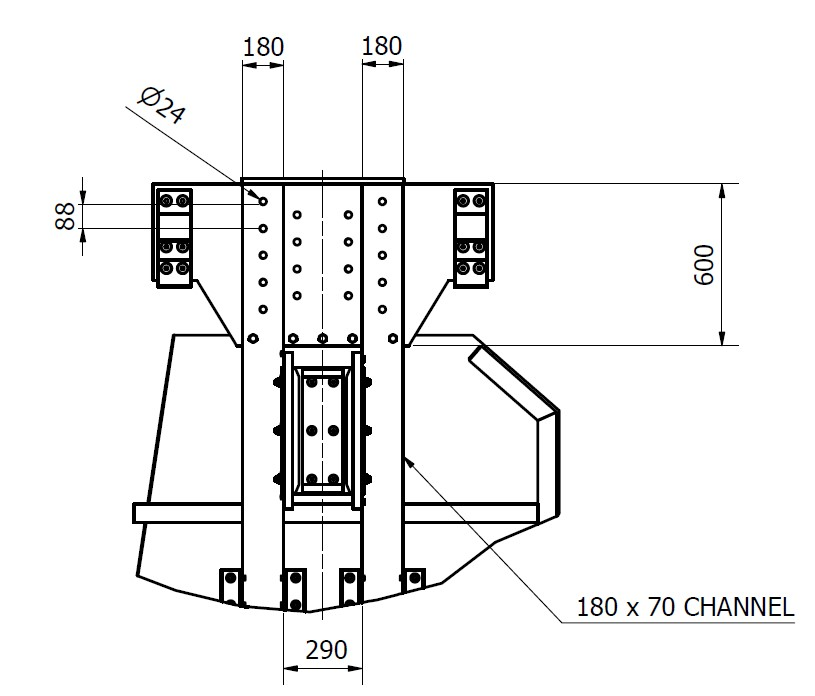
\includegraphics[width=360px]{Bridle.jpg}%
\centering%
\caption{Bridle Configuration}%
\centering%
\end{figure}

%
\textbf{Design for Emergency Loads}%
\begin{flushleft}%
\begin{minipage}{\textwidth}%
\flushleft%
\begin{tabular}{l l l l}%
Total Cross Sectional Bridle Area&$A_t$&10720&$mm^2$\\%
Total Net Cross Sectional Bridle Area&$A_e$&10048&$mm$\\%
Rope Break Force&$RBF$&2319&$kN$\\%
Tensile Resistance per Channel&$T_r = 0.85 \phi A f_y$&682.0&$N$\\%
Number of Bridless&$No.$&4&\\%
Total Tensile Resistance&$T_r$&2728.0&$N$\\%
Interaction Check&$T_u/T_r < 1$&0.85&$Pass$\\%
\end{tabular}%
\end{minipage}%
\end{flushleft}%
\newpage%
\textbf{Design for Fatigue Loads}%
\begin{flushleft}%
\begin{minipage}{\textwidth}%
\flushleft%
\begin{tabular}{l l l l}%
Cycles per Month&$Cycles$&3000&\\%
Design Life&$Design$&24&$months$\\%
Total Number of Trips&$Trips$&72000&\\%
Number of Bridle Channels&$N_b$&4&\\%
Rock during Filling&$R_d = (\alpha_v)(R)$&27000.0&$N$\\%
Permanent Load&$G_c = (m_1 + m_3 + m_4)g$&81943&$N$\\%
Major Cycle Load&$MCL = R_d + 0.25G_c$&47485.75&$N$\\%
Stress Amplitude&$\sigma_a = MCL/(N_b A_n))$&18.9&$MPa$\\%
Acceleration Cycles Load&$2A_o$&84330&$N$\\%
Stress Acceleration Increase&$\sigma_b = (2 A_o/(N_b A_n))$&8.4&$MPa$\\%
Bounding Load&$0.2R$&3600.0&$N$\\%
Stress Acceleration Increase&$\sigma_c = (0.2 R/(N_b A_n))$&0.4&$MPa$\\%
Steel Endurance Limit&$S_e$&70&$MPa$\\%
Interaction Check&$\sigma_a/S_e + \sigma_b/S_e + \sigma_c/S_e < 1$&0.4&$Pass$\\%
\end{tabular}%
\end{minipage}%
\end{flushleft}

%
\newpage

%
\section{SUMMARY}%
\label{sec:SUMMARY}%
jjjjjjjjjj

%
\end{document}